
\documentclass[a4paper,twoside]{report}
\usepackage{INScore}
\usepackage[T1]{fontenc}
\usepackage{ae,aecompl}
\usepackage{pslatex}
\usepackage{times}
\usepackage[utf8]{inputenc}
\usepackage{graphicx}
\usepackage{amssymb}
\usepackage{rail}
\usepackage{makeidx}
\usepackage{color}
\usepackage{hyperref}
\usepackage{comment}
\usepackage{multicol}
\usepackage{textcomp}


\definecolor{mycolor}{rgb}{0.384,0.0,0.145}
\hypersetup{
	colorlinks=true,
	linkcolor= mycolor
}


\setlength\parskip{\medskipamount}

\makeatletter
\railparam{\addtolength{\itemsep}{-3ex}}

%\newcommand{\toplevel}[1]	{\section{#1}}
%\newcommand{\sublevel}[1]	{\subsection{#1}}
%\newcommand{\subsublevel}[1]	{\subsubsection{#1}}

\newcommand{\toplevel}[1]	{\chapter{#1}}
\newcommand{\sublevel}[1]	{\section{#1}}
\newcommand{\subsublevel}[1]	{\subsection{#1}}

\newcommand{\fullref}[1]	{\ref{#1} p.\pageref{#1}}

\providecommand{\boldsymbol}[1]{\mbox{\boldmath $#1$}}
\newcommand{\OSC}[1]		{\texttt{#1}}
\newcommand{\values}[1]		{\texttt{#1}}
\newcommand{\oldexample}	{\hspace*{1cm}}
\newcommand{\example}		{\textbf{\hspace{-1.5cm}\textbf{\textsc{Example }}}}
\newcommand{\note}	[1]		{\vspace{2mm}\textbf{\hspace{-0.9cm}\textbf{\textsc{Note #1}}}}
\newcommand{\warning}[1]	{\vspace{2mm}\textbf{\hspace{-1.5cm}\textbf{\textsc{Warning #1}}}}

\renewcommand{\seealso}		{\textbf{See also: }}

\newcommand{\osctype}[1]	{\textbf{\texttt{{\small #1}}}}
\newcommand{\oscint}		{\osctype{int32}}
\newcommand{\oscfloat}		{\osctype{float32}}
\newcommand{\oscstring}		{\osctype{string}}
\newcommand{\rational}		{\osctype{rational}}
\newcommand{\lowTilde} 		{\texttildelow}
\newcommand{\icomment} 		{\#}

\let\olditemize\itemize
\let\oldenditemize\enditemize
\renewenvironment{itemize} 	{\olditemize \setlength{\itemsep}{1mm}}{\oldenditemize}


\setlength\parskip{2pt}
\setlength\railnamesep{-1mm}
\railterm{int32, float32, string}
\railalias{int32}{\oscint}
\railalias{float32}{\oscfloat}
\railalias{string}{\oscstring}


\definecolor{mygrey}{gray}{0.93}
\newcommand{\sample}	[1]			{\vspace{-2mm}\begin{center}\colorbox{mygrey}{
								\begin{minipage}[t]{0.9\columnwidth} 
								{\small \texttt{#1}}
								\end{minipage}}\end{center}}
\newcommand{\samplev}[1]			{\begin{center}\colorbox{mygrey}{
								\begin{minipage}[t]{\columnwidth} 
								{\small \texttt{#1}}
								\end{minipage}}\end{center}}
\newcommand{\sampleindent}	{ \hspace{0.5cm} }


\makeatother
\makeindex


\begin{document}

\title{INScore v.1.27 \\ - \\ Scripting language}

\author{D. Fober\\ GRAME\\ Centre national de création musicale\\
{\small <fober@grame.fr>} \\
%\vspace{2mm}
%ANR-08-CORD-010
}

\maketitle

%\vspace*{17.5cm}
 

{\small INScore research and development has been funded by the French National Research Agency [ANR]\\ Interlude project [ANR- 08-CORD-010] and INEDIT project [ANR-12-CORD-0009].}
  

\pagestyle{empty}
\cleardoublepage
\tableofcontents

\thispagestyle{empty}
\pagestyle{plain}

\newpage

\setcounter{page}{1}


%===============================
%:Scripting
\toplevel{INScore Scripting Language}
\label{scripting}

%===============================
%:    Introduction
\sublevel{Introduction}
\label{introduction}

INScore scripting language is based on a textual version of OSC messages, extended with variables, Javascript sections and Mathematical expressions.
INScore scripts files are expected to carry a \OSC{.inscore} extension. You can drop them to the INScoreViewer application or to any opened INScore scene.

The application or scene state can be saved (using the \OSC{save} message) as files containing textual OSC messages. These files can be edited or created from scratch using any text editor. 

%===============================
%:    Statements
\sublevel{Statements}
\label{scriptstatement}
An INScore file is a list of textual expressions. An expression is:
\begin{itemize}
\item a message: basically a textual OSC message extended to support URL like addresses and variables as parameters.
\item a variable declaration.
\item a foreign language script that may generate messages as output.
\item an end marker '\OSC{\_\_END\_\_}' to declare a script end. After the marker, the remaining part of the script will be ignored.
\end{itemize}

\index{Scripting!expressions}

\begin{rail}
expression :  
		 	message ";"
		| 	variabledecl ";"
		| 	script
		|   end
\end{rail}

Messages and variables declarations must be followed by a semicolon that is used as statements separator.

%===============================
%:    Messages
\sublevel{Messages}
\label{scriptmsgs}

Messages are basic OSC messages that support an OSC address extension scheme and relative addresses that are described below.
Messages parameters can be replaced by variables that are evaluated at parsing level. Variables are described in section \ref{scriptvar}.

Using the address extension scheme, a script may be designed to initialize an INScore scene and external applications as well, including on remote hosts.

\subsublevel{Extended OSC addresses}
\label{extaddress}





\example\\
Initializing a score and an external application listening on port 12000 and running on a remote host named \OSC{host.adomain.net}.
\sample{/ITL/scene/score set gmnf 'myscore.gmn';\\
host.adomain.net:12000/run 1;
}

Relative addresses have been introduced to provide more flexibility in the score design process. A relative address starts with '\OSC{./}'. It is evaluated in the context of the message receiver: a legal OSC address is dynamically constructed using the receiver address that is used to prefix the relative address. 

\example
\sample{the relative address \hspace*{3mm}./score \\
addressed to \hspace*{15.4mm}/ITL/scene/layer\\
will be evaluted as \hspace*{4mm}/ITL/scene/layer/score
}

The receiver context may be:
\begin{itemize}
\item the INScore application address (i.e. \OSC{/ITL}) for messages enclosed in a file loaded at application level (using the \OSC{load} message addressed to the application) or for files dropped to the application or given as arguments of the INScoreViewer application.
\item a scene address for messages enclosed in a file loaded at scene level (using the \OSC{load} message addressed to a scene) or for files or messages dropped to a scene window.
\item any object address when the messages are passed as arguments of an \OSC{eval} message (see section \fullref{miscmsgs}).
\end{itemize}

\example\\
Using a set of messages in different contexts:
\sample{score = (\\
\hspace*{5mm}./score set gmn '[a f g]', \\
\hspace*{5mm}./score scale 2.\\
);\\
/ITL/scene/l1 eval \$score;\\
/ITL/scene/l2 eval \$score;
}

\note{}\\
Legal OSC addresses that are given as argument of an \OSC{eval} message are not affected by the evaluation.


%===============================
%:    types
\sublevel{Types}
\label{scripttypes}

Using OSC, the message parameters are typed by the OSC protocol. 
With their textual version, any parameter is converted to an OSC type (i.e. int32, float or string) at parsing level.
A special attention must be given to strings in order to discriminate addresses and parameters. Strings intended as parameters must:
\begin{itemize}
\item be quoted, using single or double quotes. Note that an ambiguous quote included in a string can be escaped using a '\verb+\+'.
\item or make use of the following characters set: \OSC{[-a-zA-Z0-9]+} or \OSC{[\_a-zA-Z][\_a-zA-Z0-9]*}.
 \end{itemize}

\example \\
Different string parameter
\sample{/ITL/scene/text set txt "Hello world";  \icomment string including a space must be quoted \\
/ITL/scene/img set file 'anImage.png';  \icomment dots must be quoted too \\
/ITL/scene/foo set txt no\_quotes\_needed;
}


%===============================
%:    Variables
\sublevel{Variables}
\label{scriptvar}

A variable declaration associates a name with a list of parameters or a list of messages.
Parameters must follow the rules given in section \ref{scripttypes}. They may include previously declared variables. A message list must be enclosed in parenthesis and a comma must be used as messages separator.

\index{Scripting! variable}

\begin{rail} 
variabledecl : 'ident' '=' ( (param | variable) +
					| '(' (message + ',') ')' ) ';'
\end{rail}

\example \\
Variables declarations
\sample{color = 200 200 200; \\
colorwithalpha = \$color 100; \icomment using another variable \\
msgsvar= ( \hspace*{2.7cm}  \icomment a variable referring to a message list \\
\hspace*{1cm} localhost:7001/world "Hello world", \\
\hspace*{1cm} localhost:7001/world "how are you ?" );
}


A variable may be used in place of any message parameter. A reference to a variable must have the form \OSC{\$ident} where \OSC{ident} is a previously declared variable. A variable is evaluated at parsing level and replaced by its content.

\example \\
Using a variable to share a common position:
\sample{x = 0.5;\\
/ITL/scene/a x \$x;\\
/ITL/scene/b x \$x;
}

Variables can be used in interaction messages as well, which may also use the variables available in the interaction context (see section \fullref{interactvar}). To differentiate between a \emph{script} and an \emph{interaction} variable, the latter must be quoted to be passed as strings and to prevent their evaluation by the parser. 

\example \\
Using variables in interaction messages: \$sx is evaluated at event occurrence	and \$y is evaluated at parsing level.
\sample{y = 0.5;\\
/ITL/scene/foo watch mouseDown (/ITL/scene/foo "\$sx" \$y);
}

%===============================
%:    Environnement variables
\sublevel{Environnement variables}
\label{envvar}

Environnement variables are predefined variables available in a script context. They provide information related to the current context. Current environment variables are:
\begin{itemize}
\item \textbf{\OSC{OSName}}: gives the current operating system name. The value is among \OSC{"MacOS"}, \OSC{"Windows"}, \OSC{"Linux"}, \OSC{"Android"} and \OSC{"iOS"}.
\item \textbf{\OSC{OSId}} : gives the current operating system as a numeric identifier. Returned value is (in alphabetic order): 
\begin{itemize}
\item 1 for Android
\item 2 for iOS.
\item 3 for Linux, 
\item 4 for MacOS, 
\item 5 for Windows, 
\end{itemize}
\end{itemize}

\note\\
There is nothing to prevent overriding of an environment variable. It's the script responsibility to handle variable names collisions.


%===============================
%:    Message based parameters
\sublevel{Message based parameters}
\label{scriptmsgparam}

Similarly to message based variables (see section \fullref{msgvar}), a message parameter may also use the result of a \OSC{get} message as parameters specified like a message based variable.
The message must be enclosed in parameters with a leading \$ sign.

\index{Scripting! message based parameters}

\begin{rail} 
msgparam : '(' (message) ')'
\end{rail}

\example \\
Displaying INScore version using a message parameter:
\sample{/ITL/scene/version set  txt "INScore version is" \$(/ITL get version);}

\note{}\\
Message based parameters are evaluated by the parser. Thus when the system state is modified by a script before a message parameter, these modifications won't be visible at the time of the parameter evaluation because all the messages will be processed by the next time task. For example:\\
\sample{/ITL/scene/obj x 0.1;\\
/ITL/scene/foo x \$(/ITL/scene/foo get x);
}
x position of \OSC{/ITL/scene/foo} will be set to x position of \OSC{/ITL/scene/obj} at the time of the script evaluation (that may be different to 0.1).

%===============================
%:    languages
\sublevel{Languages}
\label{scriptlang}

\index{Scripting!javascript}
%\index{Scripting!lua}

INScore supports Javascript and Lua as scripting languages. Javascript is embedded by default (using the Qt Javascript engine). INScore needs to be recompiled to embed the Lua engine\footnote{\url{http://www.lua.org/}}. A script section is indicated similarly to a Javascript section in html i.e. enclosed in an opening \OSC{<?} and a closing \OSC{?>}.

\index{Scripting! javascript}
%\index{Scripting! lua}

\begin{rail} 
script : '<?' ('javascript' | 'lua') script '?>'
\end{rail}

The principle of using an embedded programming language in script files is the following: \emph{javascript} or \emph{lua} sections are given to the corresponding engine and are expected to produce INScore messages on output.
These messages are then parsed as if replacing the corresponding script section.

Note that INScore variables are exported to the current language environment.

\example
\sample{
<?javascript \\
\hspace*{3mm} "/ITL/scene/version set 'txt' 'Javascript v."  + version() + "';"; \\
\hspace*{1mm} ?>
}

A single persistent context is created at application level and shared to each scene.

\note Lua support is going to be deprecated and should be removed in a future release.

%===============================
%:    The Javascript objects
\subsublevel{The Javascript object}
\label{jsobj}

The Javascript engine is available at runtime at the address \OSC{/ITL/\textit{scene}/javascript}. It has a \OSC{run} method that takes a javascript string as parameter.

\index{Scripting! javascript! run}

\begin{rail} 
javascript :  'run' 'code'
\end{rail}

The \OSC{run} method evaluates the code. Similarly to javascript sections in scripts, the output of the evaluation is expected to be a string containing valid INScore messages that are next executed. 
Actually, including a javascript section in a script is equivalent to send the \OSC{run} message with the same code as parameter to the javascript object.

The Javascript engine is based on the Qt5 Javascrip engine, extended with additional functions:
\begin{itemize}
\item \textbf{\OSC{version()}} : gives the javascript engine version number as a string.
\item \textbf{\OSC{print(val1 [, val2 [, ...]])}} : print the arguments to the OSC standard output. The arguments list is prefixed by 'javascript:'. The function is provided for debug purpose.
\item \textbf{\OSC{readfile(file)}} : read a file and returns its content as a string. The file name could be specified as an absolute or relative path. When relative, the file is searched in the application current \OSC{rootPath} (see section \fullref{applmgmt}).
\item \textbf{\OSC{post(address [,...])}} : build an OSC message and post it for delayed processing i.e. to be processed by the next time task. \OSC{address} is an OSC or an extended OSC address. Optional arguments are the message parameters.
\item \textbf{\OSC{osname()}} : gives the current operating system name. Returned value is among \OSC{"MacOS"}, \OSC{"Windows"}, \OSC{"Linux"}, \OSC{"Android"} and \OSC{"iOS"}.
\item \textbf{\OSC{osid()}} : gives the current operating system as a numéric identifiant. Returned value is (in alphabetic order): 
\begin{itemize}
\item 1 for Android
\item 2 for iOS.
\item 3 for Linux, 
\item 4 for MacOS, 
\item 5 for Windows, 
\end{itemize}
\end{itemize}


\example
\sample{
<?javascript \\
\hspace*{3mm} post ("/ITL/scene/obj", "dalpha", -1);";\\ 
\hspace*{3mm} \# The message /ITL/scene/obj dalpha -1 \\
\hspace*{3mm} \# will be evaluated by the next time task. \\
?>
}

\example
\sample{
<?javascript \\
\hspace*{3mm} \# declare a function foo() \\
\hspace*{3mm} function foo(arg) \{\\ 
\hspace*{6mm}  return "/ITL/scene/obj set txt foo called with " + arg + ";"; \\
\hspace*{3mm} \} \\
?>\\
\\
\# call the foo function \\
<?javascript foo(1)?>\\
\\
\# or call the foo function using the run message \\
/ITL/scene/javascript run "foo(1)";
}

%===============================
%:Math expressions

% !TEX root = MathRef.tex

\newcommand{\mathstring}[1]		{\textit{string}(\OSC{#1})}
\newcommand{\mathstrnum}[1]		{\textit{length}(\OSC{#1})}
\newcommand{\mathsize}[1]		{\textit{size}(\OSC{#1})}
\newcommand{\op}				{$op$}
\newcommand{\todo}	[1]			{{\big [\texttt{\textbf{#1}}]}}

%===============================
%:Mathematical expressions
\toplevel{Mathematical expressions}
\label{mathExpr}

Since INScore version 1.20, mathematical expressions have been introduced as messages arguments. These expressions allows to compute values at parsing time.

%===============================
%:    Operators
\sublevel{Operators}
\label{Operators}

Basic mathematical expressions are supported. They are listed below.

\index{Math expression!operators}

\begin{rail}
mathexpr:     [1] matharg '+' matharg
			| [2] matharg '-' matharg
			| [3] '-' matharg
			| [4] matharg '*' matharg
			| [5] matharg '/' matharg
			| [6] matharg '\%' matharg
			| [7] '(' mathexpr ')'
			| [8] 'max' '(' (matharg +) ')'
			| [9] 'min' '(' (matharg +) ')'
			| [10]'(' mathbool '?' matharg ':' matharg ')'
\end{rail}

Note that \textit{matharg} could be a \textit{mathexpr} as well (see section \ref{mathargs}).

\begin{itemize}
\item \textbf{1}: addition.
\item \textbf{2}: substraction.
\item \textbf{3}: negation.
\item \textbf{4}: multiplication.
\item \textbf{5}: division.
\item \textbf{6}: modulo.
\item \textbf{7}: parenthesis, to be used for evaluation order.
\item \textbf{8}: gives the maximum value.
\item \textbf{9}: gives the minimum value.
\item \textbf{10}: conditional form: returns the first \OSC{matharg} if \OSC{mathbool} is true, otherwise returns the second one.
\end{itemize}

\example\\
Some simple mathematical expressions used as message parameters:
\sample{/ITL/scene/myObject x 0.5 * 0.2;\\
/ITL/scene/myObject y (\$var ? 1 : -1);
}

Boolean operations are the following:

\index{Math expression!booleans}

\begin{rail}
mathbool:     [1] arg
			| [2] '!' arg
			| [3] arg '==' arg
			| [4] arg '>' arg
			| [5] arg '>=' arg
			| [6] arg '<' arg
			| [7] arg '<=' arg
\end{rail}

\begin{itemize}
\item \textbf{1}: evaluate the argument as a boolean value.
\item \textbf{2}: evaluate the argument as a boolean value and negates the result.
\item \textbf{3}: check if the arguments are equal.
\item \textbf{4}: check if the first argument is greater than the second one.
\item \textbf{5}: check if the first argument is greater or equel to the second one.
\item \textbf{6}: check if the first argument is less than the second one.
\item \textbf{7}: check if the first argument is less or equal to the second one.
\end{itemize}

\example\\
Compare two variables:
\sample{/ITL/scene/myObject x (\$var1 > \$var2 ? 1 : -1);
}


%===============================
%:    Arguments
\sublevel{Arguments}
\label{mathargs}

Arguments of mathematical operations are the following:

\index{Math expression!arguments}

\begin{rail}
matharg:      [1] 'param'
			| [2] 'variable'
			| [3] 'variable' ('++' | '--')
			| [4] ('++' | '- -') 'variable' 
			| [5] 'msgvariable'
			| [6] mathexpr
\end{rail}

\begin{itemize}
\item \textbf{1}: any message parameter.
\item \textbf{2}: a variable value.
\item \textbf{3}: a variable that is post incremented or post decremented.
\item \textbf{4}: a variable that is pre incremented or pre decremented.
\item \textbf{5}: a message based variable.
\item \textbf{6}: a mathematical expression.
\end{itemize}



%===============================
%:    Polymorphism
\sublevel{Polymorphism}
\label{mathpoly}

Since INScore's parameters are polymorphic, the semantic of the operations are to be defined notably when applied to non numeric arguments. Actually, a basic OSC message parameter type is between \OSC{int32}, \OSC{float32} and \OSC{string}. However, due to the extension of the scripting language, parameters could also be arrays of any type, including mixed types (e.g. resulting from variable declarations). 

%===============================
\subsublevel{Numeric values}
\label{numbers}

For numeric arguments, automatic type conversion is applied with a precedence of \OSC{float32} i.e. when one of the argument's type is  \OSC{float32}, the result is also  \OSC{float32} (see Table \ref{table:mathopnum}).

\label{table:mathopnum}

\begin{table}[htbp]
  \centering
  \begin{tabular}{rlc}
    \hline
    arg1 & arg2 & output\\ 
    \hline
    \OSC{int32}		&  	\OSC{int32}		& \OSC{int32} \\ 
    \OSC{float32}	&  	\OSC{int32}		& \OSC{float32} \\ 
    \OSC{int32}		&  	\OSC{float32}	& \OSC{float32} \\ 
    \OSC{float32}	&  	\OSC{float32}	& \OSC{float32} \\ 
    \hline
  \end{tabular}
  \caption{Numeric operations output}
\end{table} 

%===============================
\subsublevel{Strings}
\label{strings}

For \OSC{string} parameters, operations that have an obvious semantic (like + applied to two strings) are defined (see Table \ref{table:mathopstr}) , the others are undefined and generate an error (see Table \ref{table:mathnoopstr}). 

\label{table:mathopstr}
\begin{table}[htbp]
  \centering
  \begin{tabular}{rlc}
    \hline
    operation & evaluates to & comment\\ 
    \hline
    \OSC{string} + \OSC{string} 		& \OSC{string} 						& concatenate the two strings \\ 
    \OSC{string} + \OSC{num} 			& \OSC{string} + \mathstring{num} 	& \OSC{num} is converted to string \\ 
    \OSC{num} + \OSC{string} 			& \mathstring{num} + \OSC{string} 	& " \\ 
    @max(\OSC{string} \OSC{string})		& \OSC{string} 						& select the largest string \\ 
    @min(\OSC{string} \OSC{string})		& \OSC{string} 						& select the smallest string \\ 
    \hline
  \end{tabular}
  \caption{Supported operations on strings}
\end{table} 

\label{table:mathnoopstr}

\begin{table}[htbp]
  \centering
  \begin{tabular}{rc}
    \hline
    operation & comment\\ 
    \hline
    \OSC{string} \op\ \OSC{string} 		& where \op\ is in [- * / \%]  \\ 
    \OSC{string} \op\ \OSC{num} 		& "  \\ 
    \OSC{num} \op\ \OSC{string} 		& "  \\ 
    -\OSC{string}  						&  \\ 
    prefixed or postfixed \OSC{string}  &  \\ 
    \hline
  \end{tabular}
  \caption{Non supported operations on strings}
\end{table} 

Boolean operations are supported on \OSC{string} only when both arguments are strings (see Table \ref{table:mathboolstr}). Other types combination generate an error.
	
\label{table:mathboolstr}

\begin{table}[htbp]
  \centering
  \begin{tabular}{rc}
    \hline
    boolean operation & evaluated as \\ 
    \hline
    \OSC{string} == \OSC{string} 		& regular strings comparison \\ 
    \OSC{string} > \OSC{string} 		& alphabetical strings comparison \\ 
    \OSC{string} >= \OSC{string} 		& " \\ 
    \OSC{string} < \OSC{string} 		& " \\ 
    \OSC{string} <= \OSC{string} 		& " \\ 
    \hline
  \end{tabular}
  \caption{Supported boolean operations on strings}
\end{table} 


%===============================
\subsublevel{Arrays}
\label{arrays}

For arrays, the operation is distributed inside the array elements:
\[
 arg\ op\ [v_1\ ...\ v_n]  := [arg\ op\ v_1\ ...\ arg\ op\ v_n] 
\]
or
\[ 
[v_1\ ...\ v_n]\ op\ arg  := [v_1\ op\ arg\ ...\ v_n\ op\ arg] 
\]

When both parameters are arrays, the operation is distributed from one array elements to the other array elements when the arrays have the same size and it generates an error when the sizes differ:
\[
[a_1\ ...\ a_i]\ op\ [b_1\ ...\ b_i]  := [a_1\ op\ b_1\ ...\ a_i\ op\ b_i\ ] 
\]

Boolean operations on arrays are evaluated as the logical $and$ of it's element's boolean values and generate an error when the arrays sizes differ.



%===============================
%:Score expressions
%%===============================
%:General format
\toplevel{Score expressions}
\label{scoreExpr}

\emph{Score expressions} allows to defines score objects (\OSC{gmn} or \OSC{pianoroll}) by dynamically combine various resources using a formal expression. To define such object one should use the basic \OSC{set} messages using a score expressions as arguments:

\example\\
The following example defines a \OSC{gmn} and a \OSC{pianoroll} object using score expressions, the meaning of the expression is explained further.

\sample{/ITL/scene/score set gmn expr(seq [a] [b]); \\
/ITL/scene/pianoroll set pianoroll expr(score);
}

%===============================
\sublevel{General Syntax}
\label{exprSyntax}

A score expression  always starts with \OSC{expr(} and ends with \OSC{)}, then 
2 syntaxes are handled:

\begin{rail}
EvaluableExpression: 	('expr')
						'('
						 (
						  ([1] operator score score)
						  |[2] score
						 )
						')'
\end{rail}

\begin{itemize}
\item \textbf{1}: Define an expression as an operation combining two scores. \OSC{operator} is the name of the operation used to combine them (see Section~\ref{operators} for operators list), and \OSC{score} are the arguments passed to  the operator (see Section~\ref{arguments} for arguments specification).
\item \textbf{2}: Define on expression using a single score. This syntax is useful when defining an object as a dynamic copy of an other existing object or file.
\end{itemize}
Each of these tokens can, of course, be separated by spaces, tabulations or carriage returns (allowing multiline expression definition).

When defining an object using a score expressions, INScore will parse it, construct an internal representation and finally evaluate it, reducing the formal expressions to a valid GMN string.

\example \\
Creating a guido object by sequencing two guido string
\sample{/ITL/scene/score set gmn expr( seq "[c d e]" "[f g h]");}
is equivalent to
\sample{/ITL/scene/score set gmn "[c d e f g h]";}

\sublevel{Score Operators}
\label{operators}

All the score operators of INScore make use of guido operators implemented in the GuidoAR library.
\begin{table*}[htbp]
\begin{center}
\begin{tabular}{rll}
\hline
operation & arguments		&	description \\
\hline
seq 	&	$s1$ $s2$		& puts the scores $s1$ and $s2$ in sequence \\
par 	&	$s1$ $s2$		& puts the scores $s1$ and $s2$ in parallel \\ 
rpar	&	$s1$ $s2$		& puts the scores $s1$ and $s2$ in parallel, right aligned \\
top 	&	$s1$ $s2$ 		& takes the $n$ first voices of $s1$ where $n$ is $s2$ voices count\\
bottom 	&	$s1$ $s2$ 	& cut the $n$ first voices of $s1$ where $n$ is $s2$ voices count \\
head	& 	$s1$ $s2$	& takes the head of $s1$ up to $s2$ duration \\
evhead 	&	$s1$ $s2$	& takes the $n$ first events of $s1$ where $n$ is the event's count of $s2$ \\
tail	&	$s1$ $s2$ 	& cut the beginning of $s1$ up to the duration of $s2$ \\
evtail 	&	$s1$ $s2$ 	& cut the $n$ first events of $s1$ where $n$ is the event's count of $s2$ \\
transpose 	&	$s1$ $s2$	& transposes $s1$ so its first note of its first voice match $s2$ one \\
duration 	&	$s1$ $s2$	& stretches $s1$ to the duration of $s2$  \\
			& 	& if not used carefully, this operator can output impossible to display rhythm\\
pitch 	&	$s1$ $s2$	& applies the pitches of $s1$ to $s2$ in a loop \\
rhythm 	&	$s1$ $s2$	& applies the rhythm of $s1$ to $s2$ in a loop \\
\hline
\end{tabular}
\end{center}

\end{table*}

%===============================
\sublevel{Score Arguments}
\label{arguments}

The syntax for arguments is quite permissive and various resources can be used as arguments for score expressions. In any case, when evaluating the expression, all the arguments will be reduce to GMN string so they can then be processed by the operators.
\begin{rail}
Argument: 	 GmnCode
			|(	
				( | '\&' | '$\sim$' )
				(		
					 filepath
					|ScoreObject
				)
			 )
			| 	EvaluableExpression
\end{rail}

\subsubsection{Arguments specification}
\label{argsSpec}

\begin{itemize}
\item \OSC{GmnCode} are not evaluated, passed as they are to operators. Both GMN and MusicXML string are supported.
\item \OSC{filepath}: on evaluation INScore read all the content of the file. Again, both GMN and MusicXML are supported. \OSC{filepath} handle absolute or relative path (from the scene rootPath) as well as url.
\item \OSC{ScoreObject}: Gmn code can be retreive from existing score objects (\OSC{gmn} or \OSC{pianoroll}) simply refering to them using their identifier (using absolute or relative path).
\item \OSC{EvaluableExpression}: an expression can also be used as an argument, thus simple operator can be combined together to create more complex ones. In that case the \OSC{expr} token can be omitted: parenthesis are sufficient.
\end{itemize}

\subsubsection{Arguments prefix}
\label{argsPrefix}

\begin{itemize}
\item \OSC{\&}: When triggering the reevaluation of an expression (see Section \ref{exprCmd}) only the arguments prefixed with \OSC{\&} are updated.


\item \OSC{\lowTilde}: before the first evaluation of a score expression, any \OSC{ScoreObjects} prefixed with a \OSC{\lowTilde} shall be replaced by their own expression. In other words, score expressions containing \OSC{\lowTilde} arguments will be expended with existing score expressions. This mechanism allows to compose not only scores and score expressions together.

\end{itemize}

\selayout
\example\\
Defining \OSC{/ITL/scene/score} as a copy of \OSC{/ITL/scene/simpleScore} duplicated 4 times.
\sample{/ITL/scene/simpleScore set gmn "[e \{c,g\} |]";\\
\\
/ITL/scene/score set gmn expr( \&simpleScore );\\
/ITL/scene/score set gmn expr( seq \lowTilde score \lowTilde score);\\
/ITL/scene/score set gmn expr( par \lowTilde score \lowTilde score);\\
}
\OSC{/ITL/scene/score} should look like:\\
\begin{figure}[H]
\begin{center}
 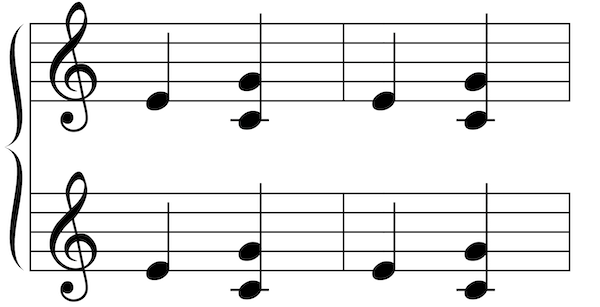
\includegraphics[scale=0.1]{imgs/seqparEnhanced}
\end{center}
\end{figure}

Querying for the expanded expression of \OSC{/ITL/scene/score} (see Section~\ref{exprCmd}) should return:
\begin{verbatim}
/ITL/scene/score expr
  expr( par
       ( seq
          &simpleScore
          &simpleScore
       )
       ( seq
          &simpleScore
          &simpleScore
       )
  )
\end{verbatim}
\smallbreak

\note{on arguments quoting} \\
Arguments using special characters (space, tabulation, parenthesis, braces...), should be simple or double quoted, otherwise quotes can be omitted.


%\pagebreak

%===============================
\sublevel{'expr' commands}
\label{exprCmd}

ITLObject defined using an evaluable expression gain access to these specific commands:

\begin{itemize}
\item \OSC{get expr}: return the expression used to define the object (before the expansion of \OSC{\lowTilde} arguments).
\item \OSC{get exprTree}: return the expanded expression

\item \OSC{expr reeval}: re-evaluate the expression, updating only the value of arguments prefixed with \OSC{\&}.
\item \OSC{expr reset}: re-evaluate the expression, updating the value of all arguments.
\item \OSC{expr renew}: reapply the definition of the object (similar to send its \OSC{set} message again)
\end{itemize}

Applied to an object which wasn't defined by an evaluable expression, all this commands will cause a bad argument error.
\smallbreak

The \OSC{renew} command reset the internal state of the evaluated variable, forcing the re-evaluation and update of every arguments in the expression. Be aware that the track of copy evaluated arguments is lost after the first evaluation, thus renewing an expression defined using copy evaluated arguments won't update these arguments to their targeted ITLObject expression. Though, static arguments added by the copy shall be renewed.


%===============================
\sublevel{newData event}
\label{exprNewData}

\OSC{newData} is triggered by any object when its value change (generally because of a \OSC{set} message). Neither trying to set an object to its actual value without changing its type, nor re-evaluating an object to its actual value will trigger newData.

Of course, the \OSC{newData} event can be used together with \OSC{reeval} to automatically update an object when the value of an other changes.

\selayout
\example\\
Creating a copy of \OSC{score}, and automatise its update when \OSC{score} is changed
\sample{/ITL/scene/score set gmn "[c e]";\\
/ITL/scene/copy set gmn expr(\&score);\\
/ITL/scene/score watch newData (/ITL/scene/copy expr reeval);
}

To avoid infinite loop when using recursion, \OSC{newData} event is delayed of one event loop, meaning that, in the previous example, during the event loop that follow \OSC{score}'s modification, \OSC{score} and \OSC{copy} are different (\OSC{copy} has not been updated yet...).

\note\\
Because newData event is delayed, if \OSC{score} experiences multiple modifications during the same event loop (because multiple \OSC{set} messages have been sent together), only his final value will be accessible when newData will be actually triggered, however the event will be sent as many times as \OSC{score} have been modified.

\note{when automatizing update}\\
For the reasons raised in the previous note, one should be very careful to delayed update when automatise \OSC{reeval} with \OSC{newData}. Indeed, in some extreme case, executing a script one line after an other won't have the same result as executing the all script at once!!

\selayout
\example\\
Creating a "score buffer", storing every state adopted by \OSC{score}
\sample{/ITL/scene/score set gmn "[c]";\\
\\
/ITL/scene/buffer set gmn "[]";\\
/ITL/scene/buffer set gmn expr(seq \&buffer (seq "[|]" \&score));\\
/ITL/scene/score watch newData (/ITL/scene/buffer expr reeval);\\
\\
/ITL/scene/score set gmn "[e]";\\
/ITL/scene/score set gmn "[g]";\\
/ITL/scene/score set gmn "[\{c,e,g\}]";
}
Won't have the same result if run line by line, or the all script as once:\\
Line by line:
\begin{figure}[H]
\begin{center}
 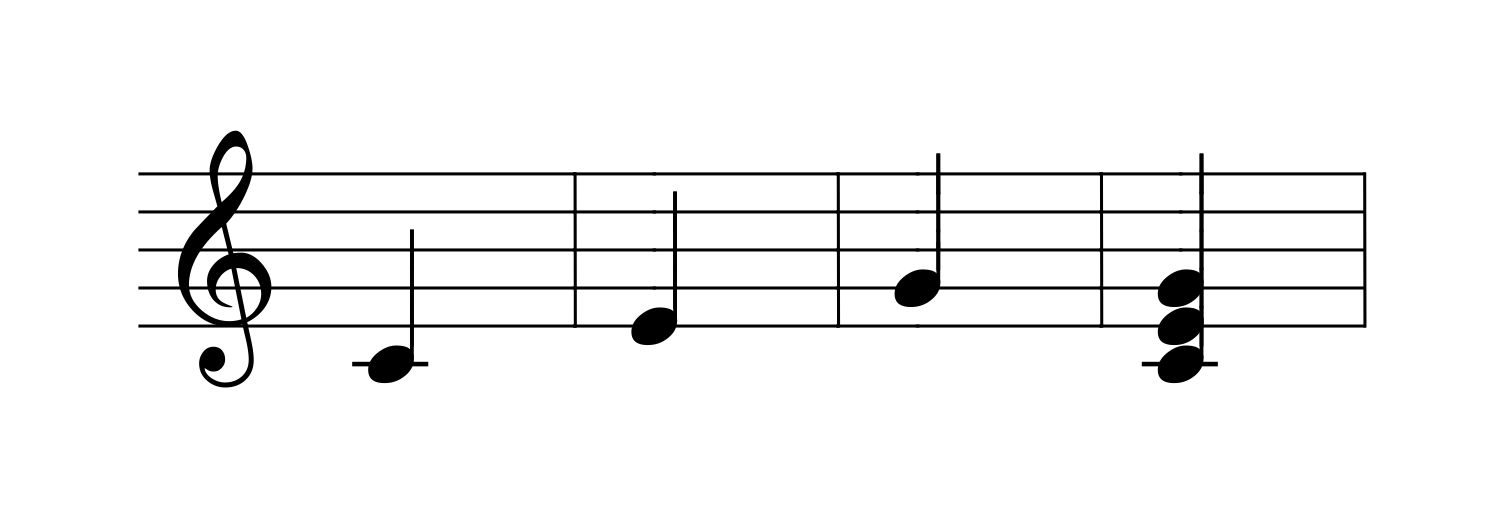
\includegraphics[scale=0.3]{imgs/autoSingleLine}
\end{center}
\end{figure}

All script lines at once:
\begin{figure}[H]
\begin{center}
 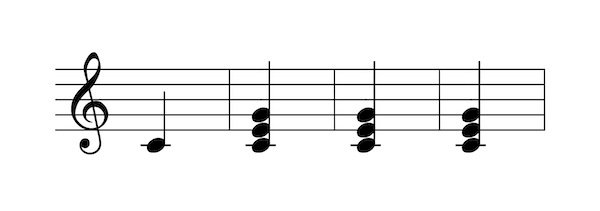
\includegraphics[scale=0.3]{imgs/autoAllScript}
\end{center}
\end{figure}

To avoid such undeterministic behaviour, one should, in this case, manually trigger \OSC{reeval} after each modification of \OSC{score}.


%===============================
%:Appendix
\toplevel{Appendices}
\label{appendices}

\sublevel{Grammar definition}
\label{yacc}

\begin{verbatim}
//_______________________________________________
// relaxed simple ITL format specification
//_______________________________________________
start        : expr
            | start expr
            ;
//_______________________________________________
// expression of the script language
//_______________________________________________
expr        : message  ENDEXPR        
            | variabledecl ENDEXPR    
            | script            
            | ENDSCRIPT            
            ;
//_______________________________________________
// javascript and support
//_______________________________________________
script        : JSCRIPT            
            ;
//_______________________________________________
// messages specification (extends osc spec.)
//_______________________________________________
message        : address                    
            | address params            
            | address eval LEFTPAR messagelist RIGHTPAR
            | address eval variable        
            ;
messagelist : message                    
            | messagelist messagelistseparator message 
            ;
messagelistseparator    : COMMA
                        | COLON
                        ;
//_______________________________________________
// address specification (extends osc spec.)
address        : oscaddress                
            | relativeaddress            
            | urlprefix oscaddress        
            ;
oscaddress  : OSCADDRESS                
            ;
relativeaddress    : POINT oscaddress        
            ;
urlprefix    : hostname  UINT            
            | STRING COLON UINT            
            | IPNUM COLON UINT            
            ;
hostname    : HOSTNAME                    
            ;
identifier    : IDENTIFIER                
            | HOSTNAME                    
            | REGEXP                    
            ;
//_______________________________________________
// parameters definitions
// eval need a special case since messages are expected as argument
eval        : EVAL                
            | variable                
            | params variable        
            | params param            
            ;
params        : sparam                
            | params sparam            
            | mathexpr                
            | params mathexpr        
            ;
variable    : VARIABLE                
            | VARIABLEPOSTINC        
            | VARIABLEPOSTDEC        
            | VARIABLEPREINC        
            | VARIABLEPREDEC        
            ;
msgvariable    : VARSTART LEFTPAR message RIGHTPAR 
            ;
param    : number                
        | FLOAT                    
        | identifier            
        | STRING                
        ;
sparam    : expression            
        | LEFTPAR messagelist RIGHTPAR    
        | script            
        ;
//_______________________________________________
// math expressions
mathexpr    : param                            
            | variable                        
            | msgvariable                    
            | mathexpr ADD mathexpr            
            | mathexpr SUB mathexpr            
            | MINUS mathexpr                
            | mathexpr MULT mathexpr        
            | mathexpr DIV mathexpr            
            | mathexpr MODULO mathexpr        
            | LEFTPAR mathexpr RIGHTPAR     
            | MIN LEFTPAR mathmin RIGHTPAR    
            | MAX LEFTPAR mathmax RIGHTPAR    
            | LEFTPAR mathbool QUEST mathexpr COLON mathexpr RIGHTPAR 
            ;
mathmin     : mathexpr                        
            | mathmin mathexpr                
            ;
mathmax     : mathexpr                        
            | mathmax mathexpr                
            ;
mathbool     : mathexpr                        
            | NEG mathexpr                    
            | mathexpr EQ mathexpr             
            | mathexpr NEQ mathexpr         
            | mathexpr GREATER mathexpr     
            | mathexpr GREATEREQ mathexpr     
            | mathexpr LESS mathexpr         
            | mathexpr LESSEQ mathexpr         
            ;
//_______________________________________________
// variable declaration
variabledecl : varname EQUAL params    
            ;
varname        : IDENTIFIER            
            ;
//_______________________________________________
// misc
number        : UINT                    
            | INT                    
            ;
//_______________________________________________
// expression declaration
expression    : EXPRESSION    
            ;
\end{verbatim}



\sublevel{Lexical tokens}
\label{lex}

\begin{verbatim}
//_______________________________________________
// numbers
//_______________________________________________
INT       a signed integer
UINT      an unsigned integer
FLOAT     a floating point number

//_______________________________________________
// hosts addresses
//_______________________________________________
// allowed character set for host names (see RFC952 and RFC1123)
HOSTNAME       : [-a-zA-Z0-9]+ 
IPNUM          :  {DIGIT}+"."{DIGIT}+"."{DIGIT}+"."{DIGIT}+

//_______________________________________________
// OSC addresses
//_______________________________________________
// allowed characters for identifiers
IDENTIFIER     : [_a-zA-Z][_a-zA-Z0-9]*
REGEXP           see OSC doc for regular expressions
OSCADDRESS

//_______________________________________________
// strings
//_______________________________________________
STRING          : ("/"|(".""."?"/")*)([^ \t\\/?:*><|"';=]+"/"?)+"."[_a-zA-Z0-9]+
                  or quoted strings that can include any character
                  quotes could be single (') or double quotes (")

//_______________________________________________
// scripting
//_______________________________________________
JSCRIPT        : <?javascript ...any javascript code... ?>
VARIABLE       : the name of a variable

//_______________________________________________
// misc.
//_______________________________________________
POINT          : '.'
VARSTART       : '$'
COLON          : ':'
COMMA          : ','
LEFTPAR        : '('
RIGHTPAR       : ')'
EQUAL          : '='
ENDEXPR        : ';'
ENDSCRIPT      : "__END__"
EVAL           : "eval"

//_______________________________________________
// score expressions
//_______________________________________________
EXPRESSION    expr( a valid score expression )
              see 'Score expressions grammar'

//_______________________________________________
// math expressions
//_______________________________________________
ADD            : '+'
DIV            : '/'
EQ             : '=='
GREATER        : '>'
GREATEREQ      : '>='
LESS           : '<'
LESSEQ         : '<='
MINUS          : '-'
MODULO         : '%'
MULT           : '*'
NEG            : '!'
QUEST          : ' ? '
SUB            : '- '
MAX            : '@max' 
MIN            : '@min'

VARIABLEPOSTDEC : $VAR--
VARIABLEPOSTINC : $VAR++
VARIABLEPREDEC  : --$VAR
VARIABLEPREINC  : ++$VAR

\end{verbatim}




\printindex

\end{document}
